\documentclass[11pt,a4paper]{article}
\usepackage[utf8]{inputenc}
\usepackage[spanish]{babel}	%Idioma
\usepackage{amsmath}
\usepackage{amsfonts}
\usepackage{amssymb}
\usepackage{graphicx} %Añadir imágenes
\usepackage{geometry}	%Ajustar márgenes
\usepackage[export]{adjustbox}[2011/08/13]
\usepackage{float}
\restylefloat{table}
\usepackage{hyperref}
\usepackage{titling}
\usepackage{minted}
\usepackage[font=small,labelfont=bf]{caption} 

%Opciones de encabezado y pie de página:
\usepackage{fancyhdr}
\pagestyle{fancy}
\lhead{}
%\rhead{}
\lfoot{Fundamentos de Redes}
\cfoot{}
\rfoot{\thepage}
\renewcommand{\headrulewidth}{0.4pt}
\renewcommand{\footrulewidth}{0.4pt}
%Opciones de fuente:
\usepackage[utf8]{inputenc}
\usepackage[default]{sourcesanspro}
\usepackage{sourcecodepro}
\usepackage[T1]{fontenc}


\setlength{\parindent}{0pt}
\setlength{\headheight}{15pt}
\setlength{\voffset}{10mm}

% Custom colors
\usepackage{color}
\definecolor{deepblue}{rgb}{0,0,0.5}
\definecolor{deepred}{rgb}{0.6,0,0}
\definecolor{deepgreen}{rgb}{0,0.5,0}

\usepackage{listings}

% Evitar guiones al final de línea.
\tolerance=1
\emergencystretch=\maxdimen
\hyphenpenalty=10000
\hbadness=10000

\pretitle{%
  \centering
  \LARGE
  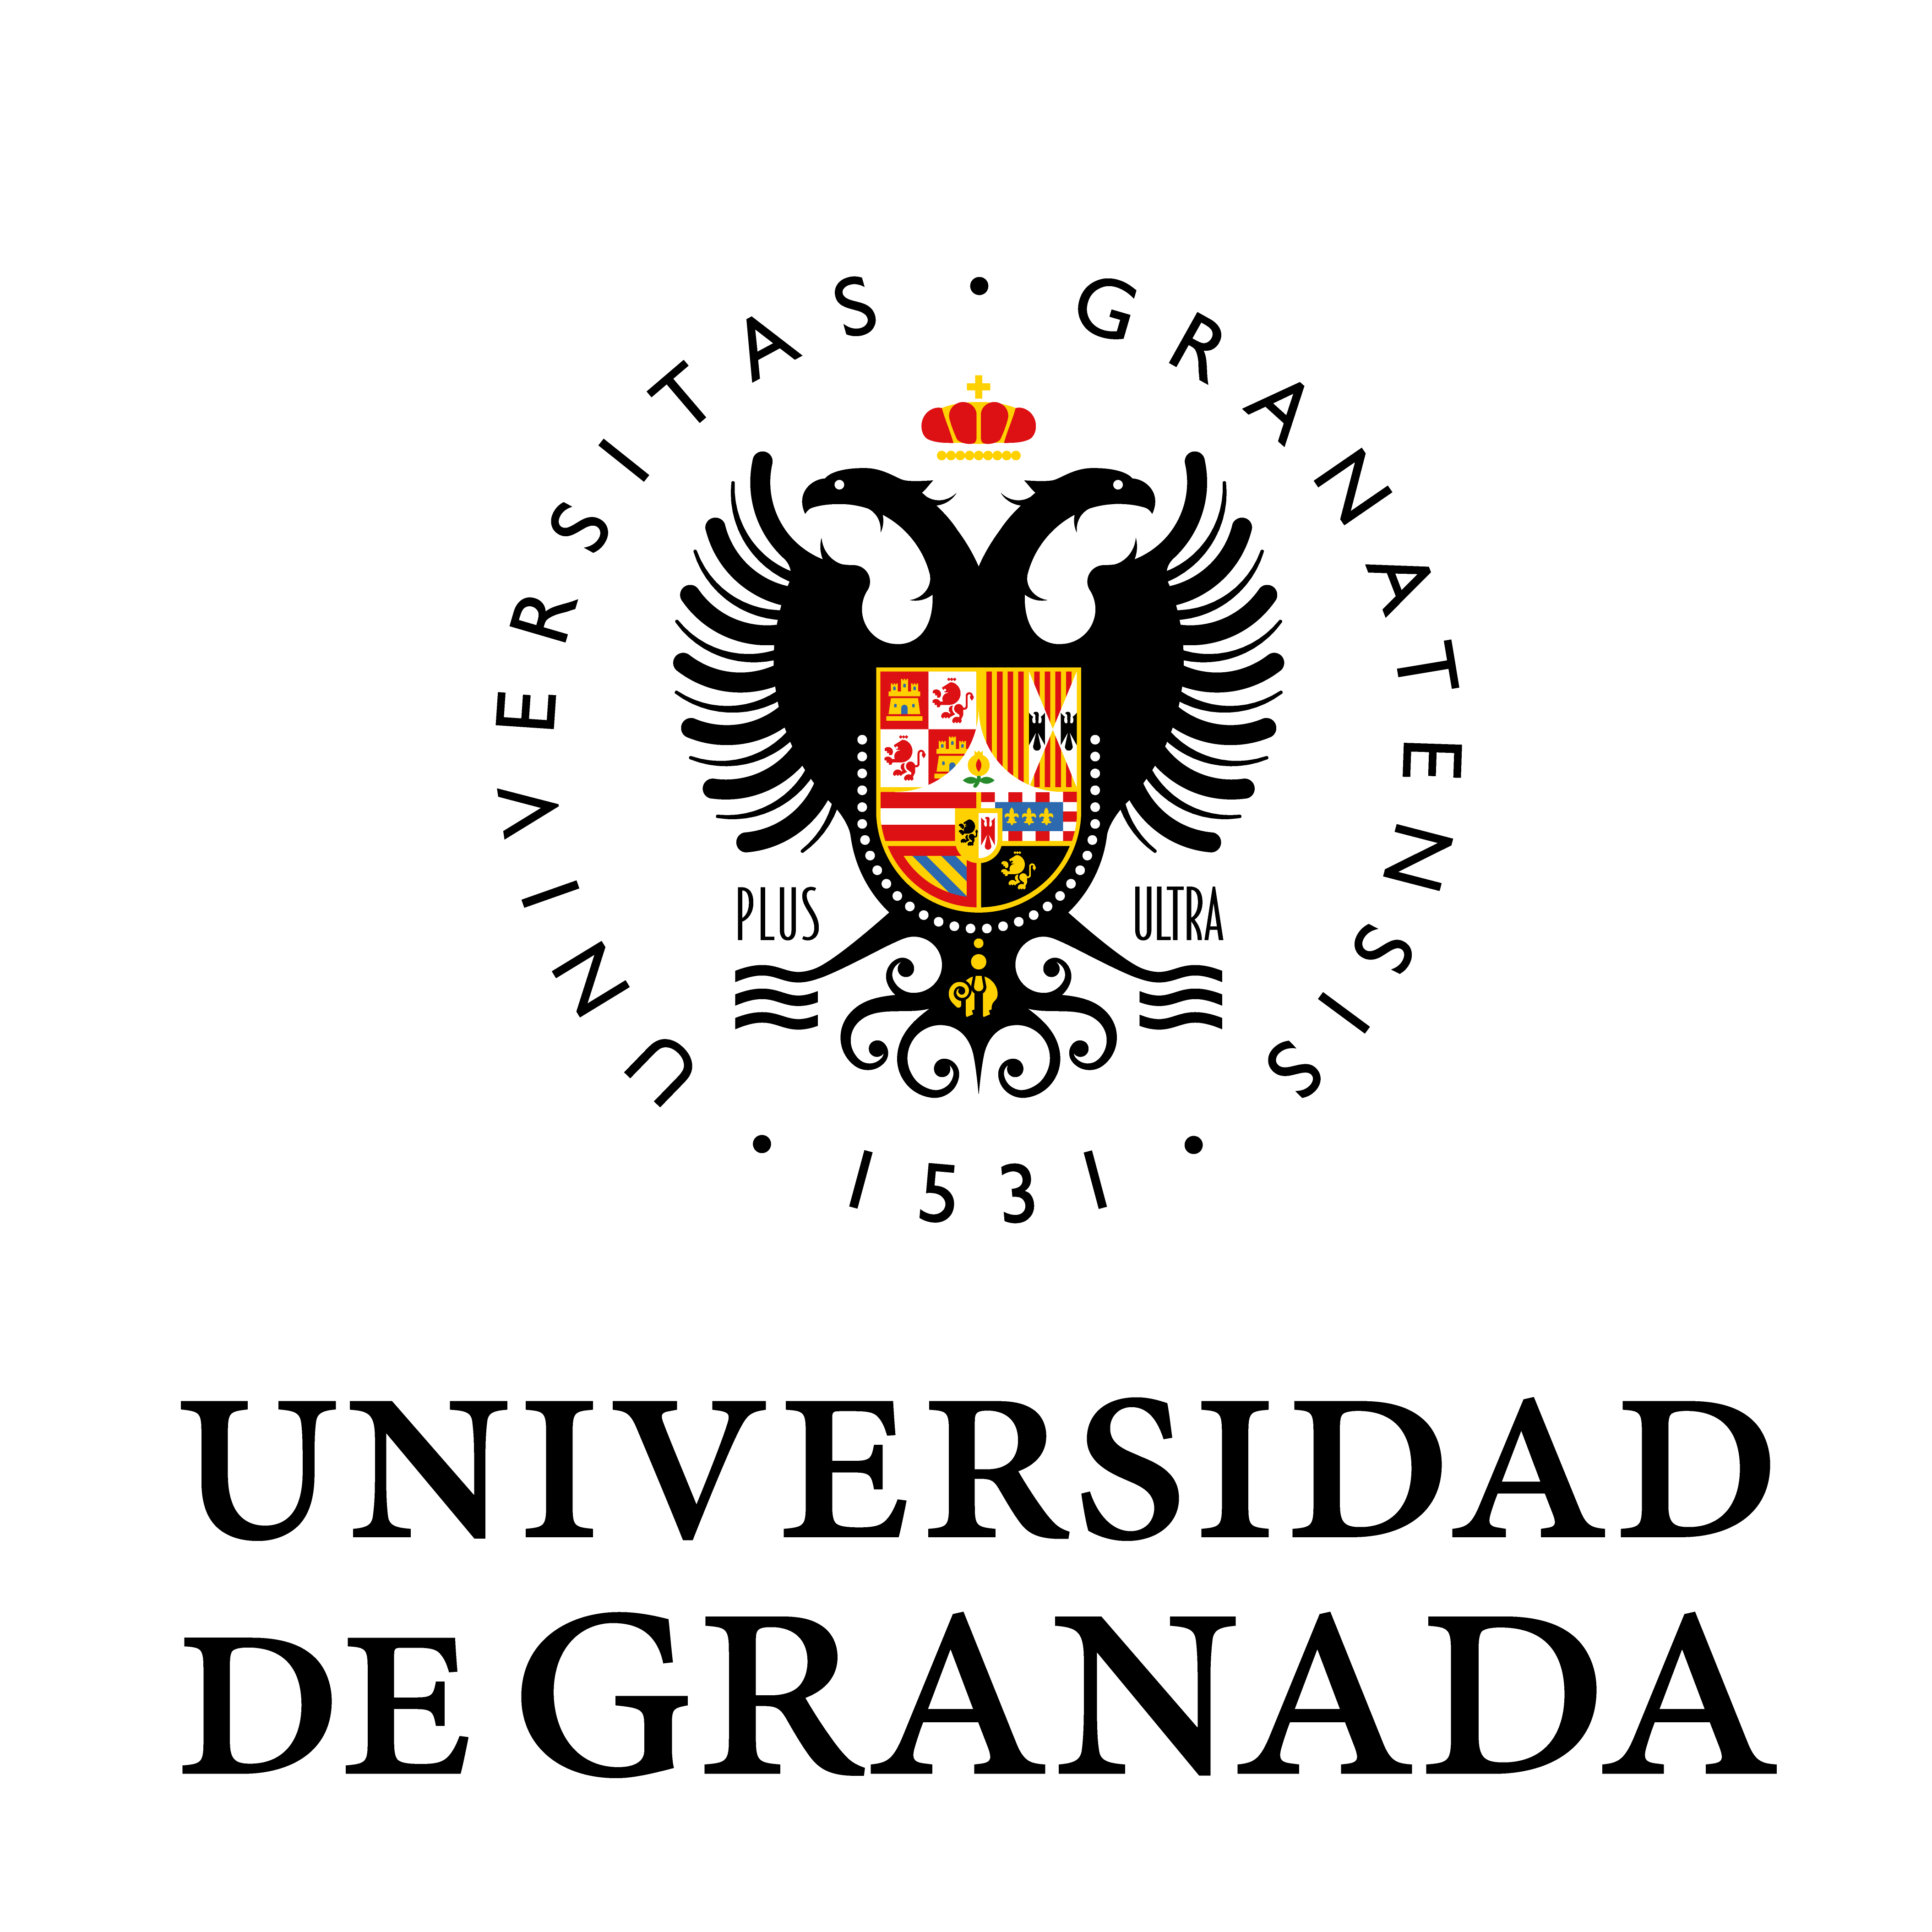
\includegraphics[scale=0.5]{img/logo.png}\\[\bigskipamount]
}
\posttitle{\begin{center} \end{center}}

\author{	Juan Ocaña Valenzuela \\ Guillermo Sandoval Schmidt }
\title{\textbf{Fundamentos de Redes} \\ 
 LoRa y LoRaWAN}

%%%%%%%%%%%%%%%%%%%%%%%%%%%%%%%%%%%%%%%%%%%%%%%%%%%%%%%%%%%%%%%%%%%%%%%%%%%%%%%
%% EL DOCUMENTO EMPIEZA AQUÍ
%%%%%%%%%%%%%%%%%%%%%%%%%%%%%%%%%%%%%%%%%%%%%%%%%%%%%%%%%%%%%%%%%%%%%%%%%%%%%%%

\begin{document}

\thispagestyle{empty}

\maketitle

\begin{center}
%\url{https://github.com/patchispatch}

Versión: 1.0
\end{center}

\newpage

\tableofcontents

\newpage

\section{LoRa}
\subsection{Qué es y cómo funciona}
\textbf{LoRa} (de Long-Range) es una tecnología inalámbrica de comunicación, como pueden ser WiFi o Bluetooth, que funciona en un rango amplio (como su nombre indica) y está basada en radio, como AM o FM.

\medskip

Desarrollada originalmente por la empresa \textit{Semtech}, aunque actualmente administrada por \textit{LoRa Alliance}, la tecnología LoRa está basada en la técnica de \textbf{modulación chirp}. La empresa la define como \textit{<<el ADN del IoT>>}. 

\medskip

En Europa utiliza las frecuencias 433 MHz y 868 MHz.

\subsection*{Modulación chirp}
La modulación chirp es una técnica de modulación por pulsos basada en el espectro ensanchado. Esta última se emplea para la transmisión de datos digitales por radiofrecuencia.

\medskip

Su fundamento básico es la transmisión a lo largo de una banda muy ancha de frecuencias, mayor que el mínimo necesario para la transmisión que deseamos realizar. Esto puede parecer un desperdicio de recursos; sin embargo, al combinarlo con sistemas que utilizan la frecuencia, maximiza su rendimiento.

\medskip

Este tipo de señal, una vez ensanchada, puede coexistir con otras señales en banda estrecha, aportando únicamente un ligero ruido.

\subsection{Ventajas y principales usos}
\begin{itemize}
\item Se ve poco afectada por las interferencias
\item Tiene poco consumo
\item Como su nombre indica, permite comunicaciones a largo alcance
\item Realiza conexión punto a punto
\end{itemize}

Estas características lo hacen excelente para su uso en redes de IoT en las que los sensores utilizados no tienen por qué disponer de corriente eléctrica.

\medskip

Algunos de sus usos podrían ser aplicaciones para \textit{Smart Cities}, aplicaciones en lugares con poca cobertura, para construir una red privada con sensores y actuadores, o para monitorizar datos médicos y datos medioambientales.

\subsection{LoRa vs. SigFox}
SigFox es otra tecnología inalámbrica centrada en IoT. A continuación, presentamos las diferencias y similitudes entre LoRa y SigFox.

\begin{itemize}
\item Ambas utilizan señales de gran alcance.
\item Ambas requieren poca energía.
\item Para usar SigFox, además de comprar el módulo correspondiente, hay que contratar un plan de suscripción.
\item LoRa puede operar de forma bidireccional, mientras que SigFox solo de manera unidireccional.
\item La API de SigFox es más simple pero menos configurable. La API de LoRa es de bajo nivel, por lo que, a pesar de que su integración sea más compleja, nos permite configurarla a nuestro gusto.
\item Ambas tecnologías ofrecen funciones de seguridad, ya que tienen comunicación cifrada. Sin embargo, ninguna de ellas ofrece comunicaciones encriptadas.
\end{itemize}

\section{LoRaWAN}
\subsection{Qué es LoRaWAN}
LoRaWAN es una especificación de redes LPWAN (Low Power Wide Area Network). Esta se encarga de unir los diferentes dispositivos LoRa, encargados de gestionar los parámetros de la conexión.

\medskip

Siguiendo la estructura del Modelo OSI, la tecnología LoRa (de la que ya hemos hablado) formaría el nivel 1 y LoRaWAN formaría el nivel 2. LoRaWAN cuenta con una arquitectura en forma de estrella, que significa que nuestros dispositivos están todos conectados a un punto central por el que deben pasar todas las comunicaciones.

\begin{center}
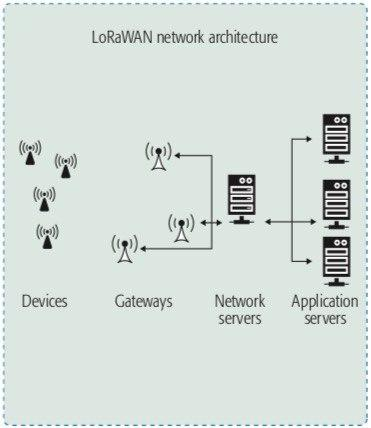
\includegraphics[scale=0.7]{img/red.jpg} \\
\small{Esquema de red LoRa}
\end{center}

\subsection{Clases de dispositivos}
LoRaWAN permite el comunicación bidireccional, aunque sea asimétrica, ya que las transmisiones hacia arriba se ven claramente favorecidas. Debido a esto, podemos diferencias 3 tipos de dispositivos, que enumeraremos como de clase A, B y C, cada uno con sus ventajas e inconvenientes.

\begin{center}
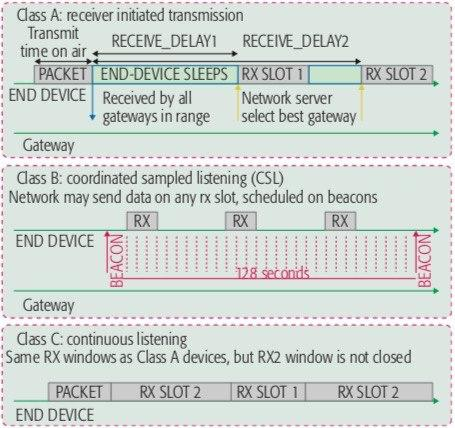
\includegraphics[scale=0.7]{img/class.jpg} \\
\small{Representación de las clases de dispositivos}
\end{center}


\subsubsection*{Clase A}
Los dispositivos de Clase A se encargan de enviar información únicamente, aunque pueden escuchar, pero de forma muy limitada (únicamente después de enviar datos a la red). Esto los hace óptimos para aplicaciones de monitorización, pues sólo envían información, y consumen poca energía. La duración de las baterías es muy elevada.

\subsubsection*{Clase B}
Esta clase de dispositivos presentan una escucha por muestreo, lo que se conoce como \textit{Coordinated Sample Listening (CSL)}. La red envía señales baliza de forma periódica, y cuando el dispositivo las recibe, comienza a escuchar durante un tiempo determinado en distintas ventanas de recepción hasta que llegue la siguiente baliza. Esto incrementa el gasto energético del dispositivo. El modelo suele aplicarse a actuadores con baterías.

\subsubsection*{Clase C}
Por último, los dispositivos de Clase C escuchan durante todo el tiempo, y tienen un gasto energético mayor. Suelen ser actuadores que requieren corriente.

\newpage

\subsection{Activación y seguridad}
La especificación de LoRaWAN dispone de una serie de identificadores para dispositivos, aplicaciones y \textit{gateways} (pasarelas), por ejemplo:
\begin{itemize}
\item \textbf{DevEUI:} identificador del dispositivo (64 bits - único)
\item \textbf{DevAddr:} dirección del dispositivo (32 bits - no único)
\item \textbf{AppEUI:} identificador de aplicación (64 bits - único)
\item \textbf{GatewayEUI:} identificador de gateway (64 bits - único)
\end{itemize}

Los dispositivos LoRaWAN disponen de un \textbf{DevEUI} asignado por el fabricante. Sin embargo, las comunicaciones se realizan utilizando el \textbf{DevAddr}.

\subsection*{Activación}
Al activar un dispositivo, formará parte de la red LoRaWAN y se comunicará con los diferentes servidores de aplicación.

\medskip

Los dispositivos pueden ser activados de dos formas:
\subsubsection*{Over The Air Activation (OTAA)}
Cuando un dispositivo se activa mediante OTAA, deriva las claves de sesión durante la operación de unión. Tanto la petición de unión como los mensajes de aceptación incluyen un código de integridad de mensaje (MIC) cifrado según la \textit{AppKey}. Así, un extremo puede verificar que el otro conoce su clave y autenticarlo de esta forma.

\subsubsection*{Activation By Personalization (ABP)}
La activación por personalización consiste en introducir manualmente la información en ambos dispositivos (\textit{hardcoded}). 

\bigskip

Independientemente del método de activación del dispositivo, se utilizan los siguientes campos:

\begin{itemize}
\item DevAddr
\item AppEUI
\item \textbf{NwkSkey:} clave de sesión de red
\item \textbf{AppSkey:} clave de sesión de aplicación
\end{itemize}

\medskip

\subsection*{Propiedades}
Las principales propiedades que cumple la seguridad de LoRaWAN son \textbf{autenticación mutua, integridad y confidencialidad}. 

\medskip

La integridad se logra gracias a un código MIC, que es usado tanto por el dispositivo como el servidor de red.

\medskip

La confidencialidad se logra ya que el tráfico de datos no solo se encripta en la interfaz over-the-air, si no que se transmite de manera segura por el núcleo del operador de red.

\medskip

El esquema de encriptado está basado en AES, lo que permite la encriptación entre el dispositivo y el servidor de red. 

\medskip

Estas características nos evitan tener que implementar otras capas de seguridad, permitiendo mantener un gasto de energía, una complejidad y un coste relativamente bajo.

\begin{center}
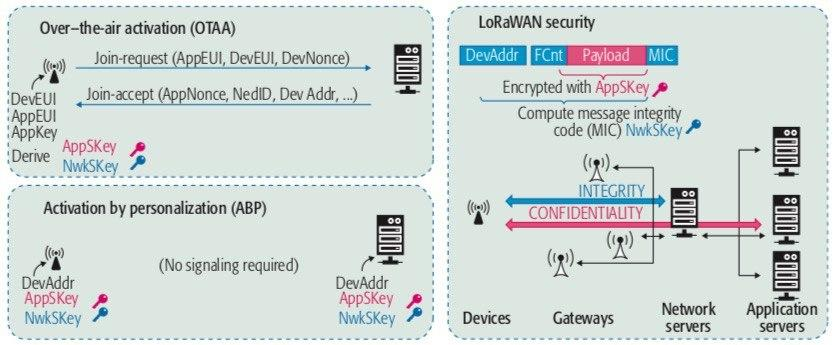
\includegraphics[scale=0.7]{img/sec.jpg} \\
\small{Esquema de la seguridad en LoRaWAN}
\end{center}

\section{Conclusiones}
LoRaWAN es una tecnología centrada en el ahorro de energía, ya que, a pesar de sus limitaciones, lo compensa con un gasto energético mínimo y un rango amplio, lo cual es idóneo para montajes de IoT que, por ejemplo, requieran monitorización de algún parámetro natural. 

\medskip

También cabe destacar que LoRa se ve afectado en espacios cerrados, pues la señal pierde mucha potencia al atravesar paredes y suelos. Por tanto, no es recomendable utilizarlo en, por ejemplo, un aparcamiento.

\medskip

En conclusión, LoRa es una tecnología barata de implementar y utilizar, y el estándar LoRaWAN permite su aplicación en el cada vez más amplio campo del \textit{Internet de las Cosas}.

\newpage

\section{Bibliografía}
\url{http://lorawan.es/}

\url{https://lora-alliance.org/about-lorawan}

\url{http://www.alfaiot.com/index.php/es/2018/05/26/que-es-lora/}

\url{https://es.wikipedia.org/wiki/Espectro_ensanchado}

\url{https://www.thethingsnetwork.org/docs/lorawan/address-space.html}

\url{https://ieeexplore.ieee.org/stamp/stamp.jsp?tp=&arnumber=8291115&tag=1}

\medskip

Agradecimientos especiales a Jorge Navarro Ortiz, profesor del Departamento de Teoría de la Señal, Telemática y Comunicaciones, por sus consejos; y a José Baena Cobos, por la cesión de un módulo RTL-SDR para realizar pruebas.
\end{document}